\subsection{Decision trees as rule generators}

A classification tree partitions the input space with axis-aligned thresholds and assigns one class to each terminal region \cite{breiman1984cart}. Each root-to-leaf path is a conjunction of interpretable conditions, so a trained tree is simultaneously a classifier and a rule generator. For imbalanced classes, accuracy rewards the majority class; the per-class recall (the fraction of each class recovered) and the recall ratio $\min(\mathrm{recalls})/\max(\mathrm{recalls})$ measure instead whether the classifier serves both classes. The acceptance criterion of this study requires a mean per-class recall above 0.6 with a balanced ratio, because an integrity classifier that misses the severe class is operationally useless regardless of its accuracy.

\subsection{Fuzzy inference with singleton consequents}

A fuzzy inference system evaluates a set of IF--THEN rules whose conditions hold to a degree between 0 and 1 given by membership functions \cite{zadeh1965fuzzy,mamdani1975experiment}. The firing strength of a rule is the minimum membership of its conditions. With singleton consequents $c_r$, the defuzzified output is the weighted average
\begin{equation}
  \hat{v}(\mathbf{x}) =
  \frac{\sum_{r} w_r(\mathbf{x})\, c_r}{\sum_{r} w_r(\mathbf{x})},
  \label{eq:fis}
\end{equation}
a Mamdani system with singleton output sets, equivalent to a zero-order Sugeno system \cite{takagi1985fuzzy}. The formulation produces a continuous output that interpolates smoothly between the rule consequents as the memberships shift, which is the property that converts a discrete severity classification into a numerical estimator.

\subsection{Nested cross-validation and leakage}
\label{sec:nested}

Model development involves selection: hyperparameters, thresholds, and design constants compete, and the winning combination is chosen because it scored best on some data. When the same data that guided the selection also produces the reported performance, the estimate is optimistically biased --- the selection has already ``seen'' the test labels, a form of information leakage \cite{varma2006bias,cawley2010overfitting}. Procedures that tune by cross-validation on the complete dataset and then refit on the same records suffer exactly this bias.

Nested cross-validation removes it with two loops (Figure~\ref{fig:nested}). The outer loop splits the data into five stratified folds; each outer test fold remains untouched during every selection and fitting step. Inside each outer training fold, an inner loop performs all the competitions: tree hyperparameters, leaf probability thresholds, and the transition-width factor of the membership functions. The complete chain then refits on the outer training fold and predicts the records of the outer test fold exactly once. The union of the five outer test folds yields out-of-fold predictions of every record, always produced by a model that never saw it. Metrics over this union estimate generalization to new monitoring points, because they reproduce the deployment situation: selection, fitting, and prediction never share records.

\begin{figure}[htb!]
  \centering
  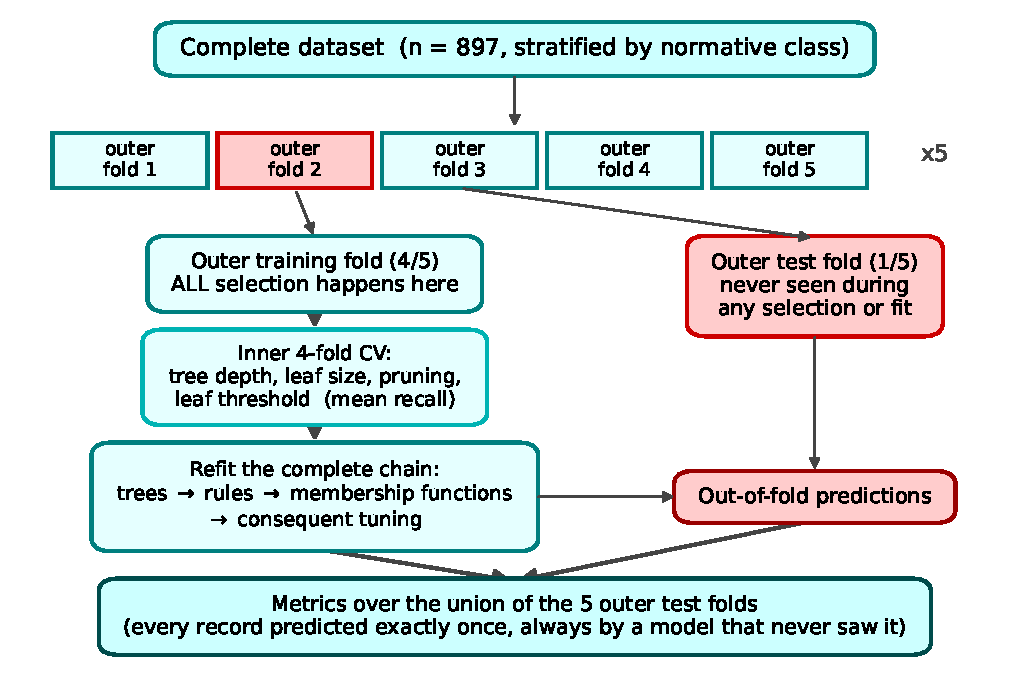
\includegraphics[width=\linewidth]{figures/nested_cv_scheme.pdf}
  \caption{Nested cross-validation protocol. Every selection step (inner 4-fold loop) and the complete refit of the chain occur inside the outer training fold; the outer test fold only receives predictions. The procedure repeats for the five outer folds, so every record is predicted exactly once by a model that never saw it.}
  \label{fig:nested}
\end{figure}
